\documentclass[oneside]{VUMIFPSkursinis}
\usepackage{algorithmicx}
\usepackage{algorithm}
\usepackage{algpseudocode}
\usepackage{amsfonts}
\usepackage{float}
\usepackage{amsmath}
\usepackage{bm}
\usepackage{caption}
\usepackage{color}
\usepackage{float}
\usepackage{graphicx}
\usepackage{listings}
\usepackage{subfig}
\usepackage{tabularx}
\usepackage{wrapfig}
\newcolumntype{P}[1]{>{\centering\arraybackslash}p{#1}}
\usepackage[%  
    colorlinks=true,
    linkcolor=black
]{hyperref}
\university{Vilniaus universitetas}
\faculty{Matematikos ir informatikos fakultetas}
\department{Programų sistemų katedra}
\papertype{Programų sistemų inžinerija II laboratorinis darbas I}
\title{Reikalavimų apibrėžimas}
\titleineng{Requirements specification}
\status{2 kurso 3 grupės studentai}
\secondauthor{Justas Tvarijonas}  
\thirdauthor{Greta Pyrantaitė}
\fourthauthor{Rytautas Kvašinskas}
\author{Tomas Kiziela}

\supervisor{Audronė Lupeikienė, M. Darbuot., Dr.}
\date{Vilnius – \the\year}


\bibliography{bibliografija}

\begin{document}
\maketitle
\tableofcontents

\section{Įžanga}
Mūsų komanda gavo kitos komandos pirmame semestre(PSI I) paruoštą slidinėjimo kurorto projektą. Šiame darbe sieksime toliau plėtoti ir keisti šį projektą. Toliau vystatnt projektą keisis daugumas dalių. Siekiant padaryti gerą produktą kai kurios  dalys bus pašalindos ir pridėtos naujos. Pirmame semestre projektuojant dėmesys buvo skiriamas klasikinei projektavimo paradigmai. Šiame darbe projektą rašysime pasinaudodami ICONIX principu, projektuojant dėmesys bus skiriamas GUI sudarymo ir iš to išplauks sistemos projektavimas ir sandara. 

\section{Reikalavimai}
Šioje dalyje bus pateikti funkciniai bei nefunkciniai reikalavimai sistemai. Stengsimės prisilaikyti ,,užsakovų"(grupės iš kurios gavome jų darbą) reikalavimus tačiau siekiant sukurti geresnę sistemą pridėsime kaikuriuos savo sugalvotus reikalavimus arba ignoruosime mums pateiktus reikalavimus. 

\subsection{Reikalavimų pataisymai}
	\begin{itemize}
		\item{X - ištrintas}
		\item{M - pakeitas}
	\end{itemize}


\begin{table}[htbp]

\begin{tabularx}{1\textwidth}{  |P{1cm}|X|P{1.5cm}|p{3.5cm}|X| }  \hline
	Nr. & Pradiniai reikalavimas &  Pakeitimo tipas & Klaidos aprašas  & Naujas reikalavimas \\ \hline
	FR & ,,Žetonas" seka vartotojo laiką praleistą trasoje & M & Pakeistas neaiškus daiktavardis & Sekimo prietaisas seka vartotojo laiką praleista trasoje \\ \hline
	FR & ,,Žetonas" skaičiuoja greičiausią laiką, per kurį vartotojas įveikia trasą & M & Pakeistas neaiškus daiktavardis & Sekimo prietaisas fiksuoją greičiausią laiką, per kurį vartotojas įveikė trasą \\ \hline
	FR & Vartotojo trasų laikai rodomi internetinėje aplikacijoje & N & NaN & NaN \\ \hline
	

	
	

\end{tabularx}

	
\end{table}

\subsection{Slidininko sekimas realiu laiku}

\begin{table}[htbp]

\begin{tabularx}{1\textwidth}{ |P{2.5cm}|X|P{3cm }| }  \hline
	Nr. & Reikalavimai & Prioritetas \\ \hline
	FR 1 & Sistema leidžia vartotojui už paslaugas atsiskaityti e-bankininkyste & 10 \\ \hline
	FR 2 & Vartotojo prieeigos prie pramogų prieinamumas nustatomas naudojant pirštų antspaudą & 8 \\ \hline
	
	
	
	FR 3& Sistema seka vartotojų poziciją specialaus žetono pagalba, kurį gauna kiekvienas vartotojas apsilankęs kurorte(Vieta sekama tik gavos vartotojo sutikimą) & 8  \\ \hline
	FR 4 & ,,Žetonas" seką vartotojo laiką praleista trasoje & 8 \\ \hline
	FR 5 & ,,Žetonas" skaičiuoją greičiausią laiką per kurį vartotojas įveikia trasą &  8 \\ \hline
	FR 6 & Vartotojo trasų laikai rodomi internetinėje aplikacijoje & 7 \\ \hline 
	

\end{tabularx}

	
\end{table}


\section{Struktūrinis dalykinės srities modelis}
\subsection{Reikalavimų veiksmažodžiai}
	Kuriant dalykinės srities modelį pagal ICONIX pirmas žingsnis yra iš pateiktų(sukurtų) reikalavimų išrinkti veiksmažodžius ir iš jų sudaryti dalykinės srirties modelį. Iš  dabar turimų reikalavimų galime išskirti šiuos daiktavardžius:
	\newline
	\newline
	Sistema, vartotojas,  pozicija, kurortas, žemėlapis, teritorija, trasas, informacija, užimtumas, rekordas, laikas, greičių lentelė. 
	\newline
	\newline
	Sutvarkius šios daiktavardžius galime pradėti brėžti domain model. 
\begin{figure}[H]
		\centering	
	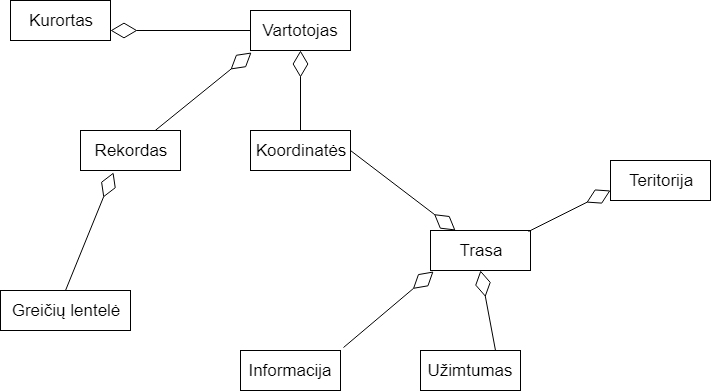
\includegraphics[width=18cm,height=20cm,keepaspectratio]{DomainModel.png}
	\caption{Domain model}
	\label{fig:Domain model}
\end{figure}
\begin{figure}[H]
		\centering	
	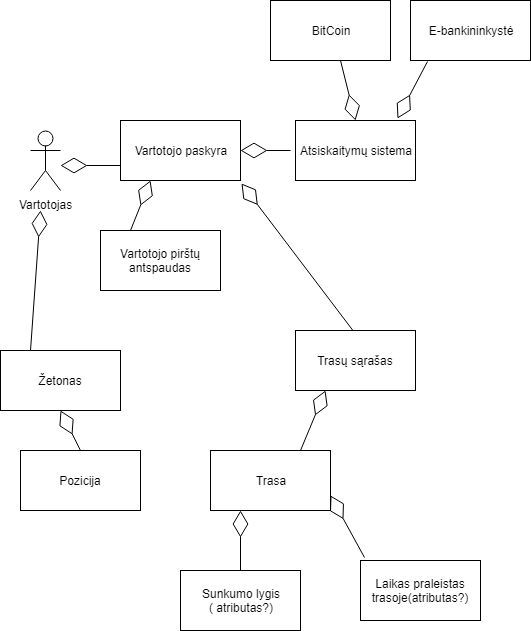
\includegraphics[width=18cm,height=20cm,keepaspectratio]{Domain2.png}
	\caption{Domain model}
	\label{fig:Domain model}
\end{figure}
Sudarius domain modelio drafta galime pradėti braižyti use case diagramą ir GUI darftini variantą. Ne viskas kas bus use case diagramoje yra domanin model diagramoje bet vėliau jis bus papildytas.



Use case draftas

\begin{figure}[H]
		\centering	
	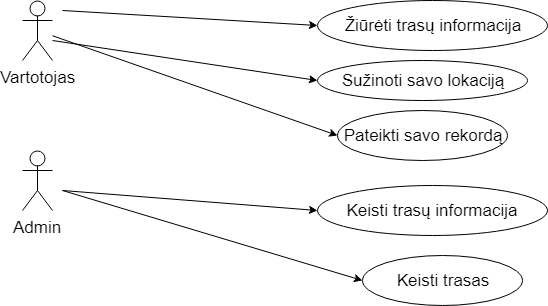
\includegraphics[width=18cm,height=20cm,keepaspectratio]{UseCase.png}
	\caption{Use case}
	\label{fig:Use case}
\end{figure}

\begin{table}[htbp]

\begin{tabularx}{1\textwidth}{ |P{17cm}|}  \hline

Pagrindinis scenarijus \\ \hline
Vartotojas prisijungia prie savo paskyros ir paspaudžia mygtuką ,,Atsiskaityti už paslaugas". Sistema pateikia pasirinkimą mokėti per E-bankininkystę arba BitCoin pervedimu. Vartotojas pasirenka norimą pasirinkimą \\ \hline
Alternatyvus scenarijus \\ \hline
Vartotojas pasirenka norimą apmokėjimo būdą, tačiau pasirinkas apmokėjimo būdas nėra pasiekiams. Vartotojui parodoma informacinę žinutę apie nepasiekiamą galimybė ir jis nukreipiamas atgal į apmokėjimo langą \\ \hline





\end{tabularx}

	
\end{table}



GUI draftas
\begin{figure}[H]
		\centering	
	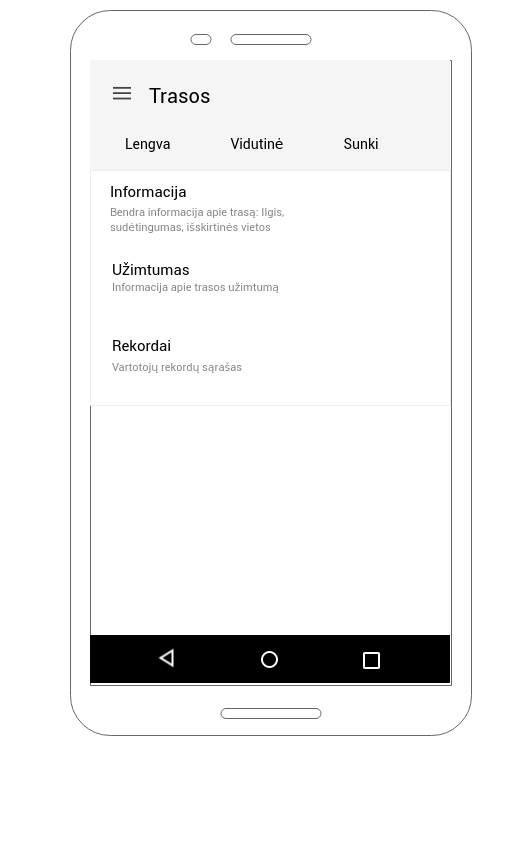
\includegraphics[width=18cm,height=20cm,keepaspectratio]{GUI.png}
	\caption{GUI}
	\label{fig:GUI}
\end{figure}









 
	

\section{Užduotys}

\section{Reikalavimų specifikacijos, dalykinės srities modelio ir užduočių diagramos peržiūros rezultatai}

\section{Išvada}

\section{Asmeninis darbo indėlis}

\section{Žodynas}


	
	





\end{document}